
\documentclass{article}
\usepackage[margin=1.0in]{geometry}
\usepackage{color}
\usepackage{caption}
\usepackage{hyperref}
\usepackage{csquotes}
\usepackage{amsmath}
\usepackage{amssymb}
\usepackage{soul}
\usepackage{changepage}
\usepackage{alg}
\usepackage{graphicx}
\usepackage{grffile}
\graphicspath{ {./} }
\usepackage{listings}
\lstset{aboveskip=3mm, belowskip=3mm, showstringspaces=false, columns=flexible, basicstyle={\small\ttfamily}, numbers=none, breaklines=true, breakatwhitespace=true, tabsize=3}

\usepackage{newlfont}
\usepackage{program}
\catcode`\_\active

\newcommand{\define}[1]{{\sc Definition.} \textbf{#1}: }
% \newcommand{\forcenewpage}{\clearpage \newpage \mbox{~} \clearpage \newpage}
\newcommand{\forcenewpage}{\clearpage \newpage}

\begin{document}
\begin{center}{\huge   Benchmarking Google Translate }\\[0.4cm]{\large  Philosophy of Computation Lab IV }\\[0.75cm]{\large  Henry Blanchette }\\[0.5cm]{\large  April 5, 2019 }\\[1.0cm]\end{center} \section{Introduction}


In this lab, I benchmarked Google Translate's (GT) performance on a multi-lingual translation task.
The goal was to measure roughly how well GT performed at difficult translation tasks and how language-choice and transcript-style affected the performance.




For input transcripts, I used several English transcripts in writing styles ranging from old-English prose to patent specification.
This variety is meant to tease out possibly effects that (1) some writing styles have on GT's ability to translate English phrases across many languages at a time due to the commonality of their grammatical and semantical structures.





For languages, I picked from the top and bottom of the ranking of languages by number of native speakers.
Each group is focused on in its own experiment (experiments 1 and 2).
This choice of languages is meant to emphasize any differences that are yielded in GT's performance by the commonality of the languages used in terms of how many examples exist for the GT algorithm to train on. This is, of course, allowing the reasonable assumption that training examples commonality roughly correlates with number of native speakers.


\section{Transcript Setup}


I selected transcript sections that reflect a variety of writing styles, including modern English, English, technical writing, storytelling, and English translated from other languages. The full text of each transcript can be found in the appendix.




\vspace{1em} \noindent
Transcripts:
\begin{enumerate}
  \item[T1.] The Bible, Genesis
  \item[T2.] Melville's Moby Dick, Chapter 1
  \item[T3.] Mariam-Webster English Dictionary, definition of Abdicate
  \item[T4.] Bedau's patentsample.txt
  \item[T5.] Shakespeare's Henry IV, Part 1
\end{enumerate}

\section{Translation task}


Start with a sequence of languages $L_0, \dots, L_n$ and a transcript in $L_0$, called the \textit{original transcript.}
GT translates the $L_0$-transcript to $L_1$, and then translates the resulting $L_1$-transcript to $L_2$, and so on until the transcript has been translated to $L_n$.
At the end, there is left a $L_n$-transcript.
Then, GT translates this $L_n$-transcript back to $L_0$ - the result is the \textit{processed transcript}.
The differences between the original and processed transcripts are measured to rate GT's success at this task.
The goal of this scoring is to rate GT according to how well it preserve the meaning and grammatic structure of the original transcript.


\section{Translation Success Measure}


I rated GT's success at the task by how close the processed transcript was to the original transcript in terms of meaning and grammar. For each of these dimensions, I categorized an ranking of ordered performance classes.




\textbf{Grammar} is how properly-constructed the processed transcript is according to the rules of $L_0$ and the grammatical structure of the original transcript.
The following are the classes of grammar performance I partitioned in order of increasing success.
They are meant to be ``evenly spaced'' in the space of deviations from the exact grammar and structure of the original transcript.
\begin{align*} \begin{array}{r|l}
\text{Grammar Class} & \text{Description} \\ \hline
1 & \text{completely confused} \\
2 & \text{mostly confused} \\
3 & \text{often confused} \\
4 & \text{sparsely confused} \\
5 & \text{effectively perfect}
\end{array} \end{align*}




\textbf{Meaning} is how close the processed transcript is to the original transcript in meaning.
The following are the classes of meaning performance I partitioned in order of increasing success.
They are meant to be ``evenly spaced'' in the space of deviations from reflecting the exact meaning of the original transcript.
\begin{align*} \begin{array}{r|l}
\text{Meaning Class} & \text{Description} \\ \hline
1 & \text{irrelevant} \\
2 & \text{sparsely relevant} \\
3 & \text{often relevant} \\
4 & \text{mostly accurate} \\
5 & \text{effectively perfect} \\
\end{array} \end{align*}





The \textbf{Euclidean Total}, $E$ is a combination of the grammar and meaning scores according the Euclidean distance formula:
\begin{align*}  E(g,m) := \sqrt{(5-g)^2 + (5-m)^2}  \end{align*} \vspace*{0.1cm}
The motivation for this score is the conception of the grammar and meaning scores as being measures along orthogonal feature axes.
So, the distance in this 2D space from $(0,0)$ represents how far from the perfect translation the processed transcript is.
A lower $E$ indicates a better translation.
The assumption that the grammar and meaning axes are orthogonal is likely false, but it is a useful approximation.


\section{Predictions}


In regards to language speaker counts, I hypothesized that GT will perform better on these languages than the languages in Experiment 2 because I assume that (1) having more native speakers correlates with having more training data for GT's algorithms, and (2) having more data to train on yields a more accurate GT in the ways measured by this experiment. Assumption 1 seems very likely in general, but assumption 2 maybe depends heavily on how exactly GT works and whether it actually works well at all.





In regards to transcript style, I hypothesized that GT will perform better the more technical and less artsy the transcript. For example, I think that it will not well-maintain neither the grammatical structure nor meaning of the Shakespeare prose because it contains analogies and uncommon grammatic structures.



%\forcenewpage
\section{Experiment 1: Well-Documented Language Translation Ring}\subsection{Language Setup}


I selected from the top 5 languages (without English) by native speaker count. The following are the languages used in this experiment in order of decreasing native speakers count: Chinese (simplified), Spanish, Hindi, Arabic, Portuguese.


\subsection{Experimental Design}


I ran each transcript through the following trials, where the selected languages and their order was chose randomly:
\begin{enumerate}
\item[] Trial 1: Chinese $\rightarrow$ Arabic $\rightarrow$ Spanish $\rightarrow$ Portuguese $\rightarrow$ Hindi
\item[] Trial 2: Hindi $\rightarrow$ Chinese $\rightarrow$ Portuguese $\rightarrow$ Arabic $\rightarrow$ Spanish
\item[] Trial 3: Hindi $\rightarrow$ Spanish $\rightarrow$ Arabic $\rightarrow$ Chinese $\rightarrow$ Portuguese
\item[] Trial 4: Chinese $\rightarrow$ Arabic $\rightarrow$ Spanish $\rightarrow$ Portuguese $\rightarrow$ Hindi
\item[] Trial 5: Arabic $\rightarrow$ Chinese $\rightarrow$ Portuguese $\rightarrow$ Spanish $\rightarrow$ Hindi
\end{enumerate}


\subsection{Results}


The full text of the results can be found in the appendix.
The summarization of the results are recorded in figures 1 and 2.



\begin{figure}[h]
\centering
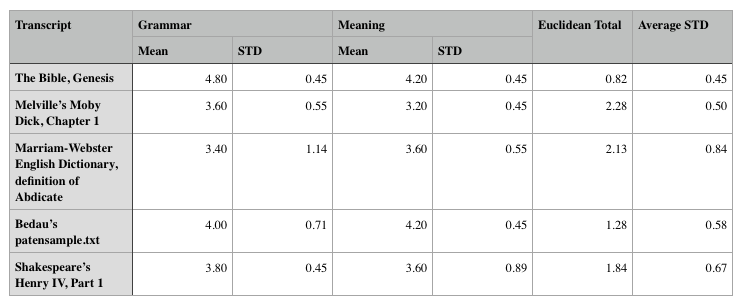
\includegraphics[width=15cm,keepaspectratio]{images/exp1-results-table.png}
\captionsetup{labelformat=empty} \caption{Figure 1. Experiment 1: Results Table.}
\end{figure}

\begin{figure}[h]
\centering
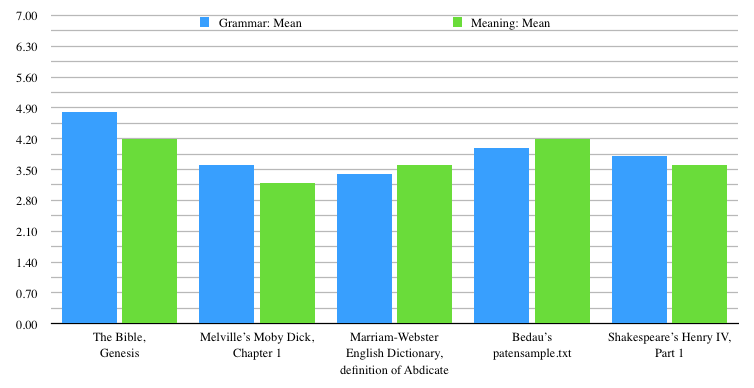
\includegraphics[width=15cm,keepaspectratio]{images/exp1-results-chart.png}
\captionsetup{labelformat=empty} \caption{Figure 2. Experiment 1: Results Chart.}
\end{figure}

%\forcenewpage
\section{Experiment 2: Under-Documented Language Translation Ring}\subsection{Language Setup}


I selected from the bottom 5 languages by native speaker count that Google Translate supports. The following are the languages used in this experiment in order of decreasing native speaker count: Nepali, Sinhala, Greek, Hungarian, Zulu.




%\forcenewpage
\subsection{Experimental Design}


I ran each transcript through the following trials, where the selected languages and their order was chose randomly:




\begin{enumerate}
\item[] Trial 1: Zulu $\rightarrow$ Hungarian $\rightarrow$ Nepali $\rightarrow$ Sinhala $\rightarrow$ Greek
\item[] Trial 2: Nepali $\rightarrow$ Hungarian $\rightarrow$ Greek $\rightarrow$ Sinhala $\rightarrow$ Zulu
\item[] Trial 3: Nepali $\rightarrow$ Sinhala $\rightarrow$ Zulu $\rightarrow$ Greek $\rightarrow$ Hungarian
\item[] Trial 4: Sinhala $\rightarrow$ Greek $\rightarrow$ Nepali $\rightarrow$ Zulu $\rightarrow$ Hungarian
\item[] Trial 5: Hungarian $\rightarrow$ Greek $\rightarrow$ Sinhala $\rightarrow$ Zulu $\rightarrow$ Nepali
\end{enumerate}

\subsection{Results}


The full text of the results can be found in the appendix.
The summarization of the results are recorded in figures 3 and 4.



\begin{figure}[h]
\centering
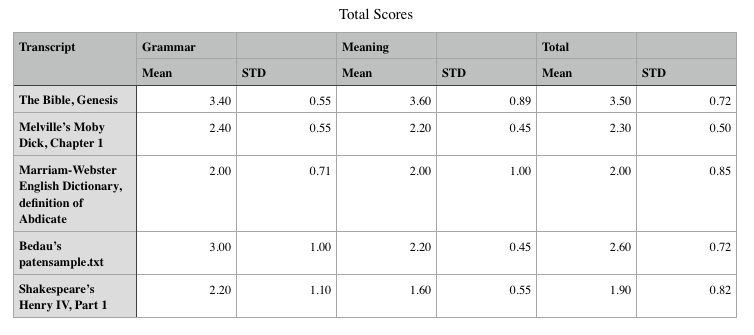
\includegraphics[width=15cm,keepaspectratio]{images/exp2-results-table.png}
\captionsetup{labelformat=empty} \caption{Figure 3. Experiment 2: Results Table.}
\end{figure}

\begin{figure}[h]
\centering
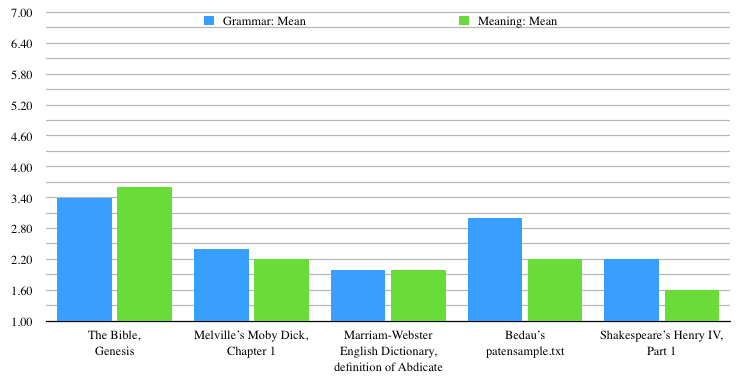
\includegraphics[width=15cm,keepaspectratio]{images/exp2-results-chart.png}
\captionsetup{labelformat=empty} \caption{Figure 4. Experiment 2: Results Chart.}
\end{figure}

\forcenewpage
\section{Analysis}\subsection{Comparing Languages}


Figure 5 records the differences between experiments of the score means for all features of each transcript used.
The \textit{difference} of the mean score for feature $F$ is calculated by subtracting the mean of $F$ in experiment 1 from the mean of $F$ is experiment 2.



\begin{figure}[h]
\centering
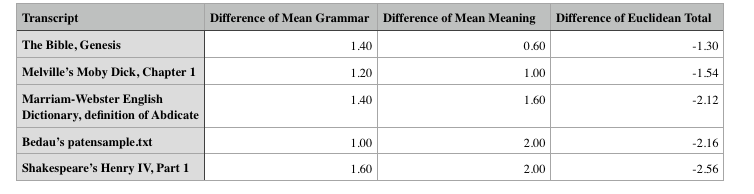
\includegraphics[width=15cm,keepaspectratio]{images/lang-diffs-all-table.png}
\captionsetup{labelformat=empty} \caption{Figure 5. Table of the differences between experiments of the means for all features of each transcript.}
\end{figure}



The results show that GT's performance with uncommon languages (the languages used in experiment 2) scored on average 1.32 points lower in grammar, 1.44 points lower in meaning, and 1.94 points higher in Euclidean total than GT's performance with common languages (the languages used in experiment 1). So as hypothesized, GT performed much worse with languages for which there is little training data in comparison to languages for which there is vast amounts of training data. In the range of the Euclidean total this is the significant drop of $  1.94/ \sqrt{50} \approx 27.4\%  $ of the total range.





This drop in performance is very consistent across the different transcripts, which suggests that this is indeed the observation of a systematic effect rather than a random bias in GT's performance; the standard deviations in the score differences are 0.23, 0.62, and 0.51 for grammar, meaning and Euclidean total respectively.





This data corresponds well to my subjective experience of reading the processed transcripts. There was a clear qualitative drop in performance when I transitioned from experiment 1 to experiment 2; most common grammatical structures and words with several meaning were maintained in experiment 1 but were almost always completely lost in experiment 2. For example, ``My liege, this haste was hot in question'' from Shakespeare was caught pretty well in experiment 1 but was almost always echoed as something to do with heat or questioning in experiment 2, such as ``My sleep was a sudden heat'' in trial 1. That example sounds like it could be an idiom in some language alien to me, but it definitely does not match Shakespeare.



\begin{figure}[h]
\centering
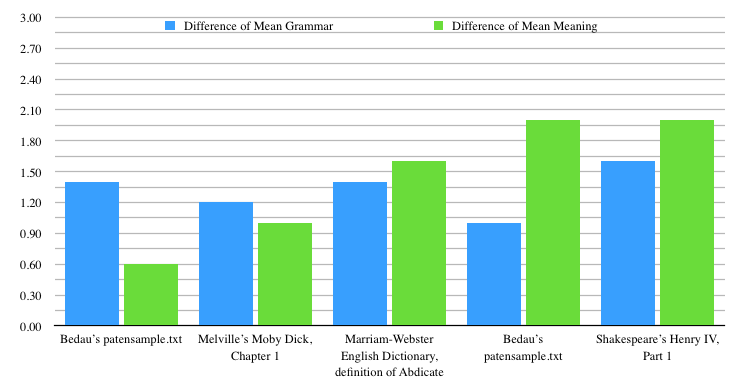
\includegraphics[width=15cm,keepaspectratio]{images/lang-diffs-grammar-meaning-chart.png}
\captionsetup{labelformat=empty} \caption{Figure 6. Chart of the differences between experiments of the means for grammar and meaning scores of each transcript.}
\end{figure}

\begin{figure}[h]
\centering
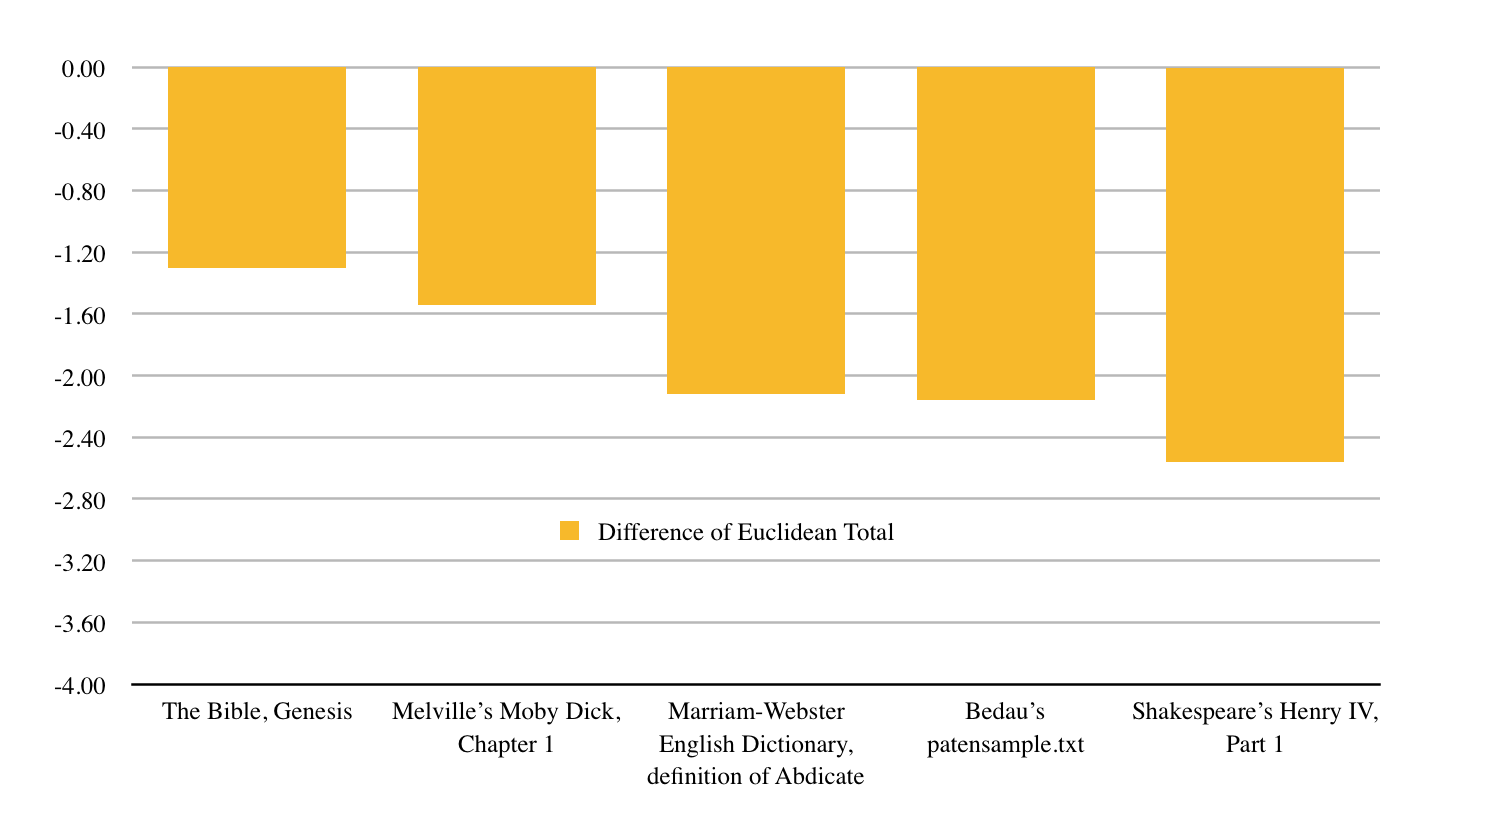
\includegraphics[width=15cm,keepaspectratio]{images/lang-diffs-euclid-chart.png}
\captionsetup{labelformat=empty} \caption{Figure 7. Chart of differences between experiments of the means for the Euclidean total score of each transcript.}
\end{figure}
\subsection{Comparing Transcripts}


Figure 8 records the differences between transcripts of their mean scores for all features for experiment 1 and 2. 
The transcripts in order of increasing mean Euclidean total are:


\begin{enumerate}
\item The Bible, Genesis


\item Beadau's patentsample.txt


\item Melville's Moby Dick, Chapter 1


\item Shakespeare's Henry IV, Part 1


\item Marriam-Webster English Dictionary, definition of Abdicate

\end{enumerate}
\begin{figure}[h]
\centering
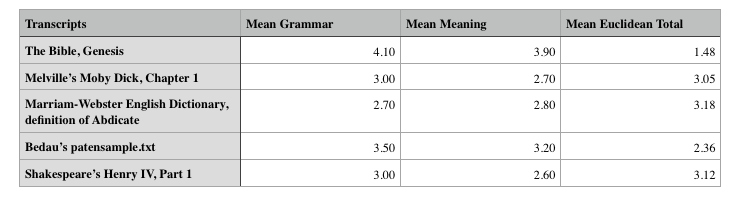
\includegraphics[width=15cm,keepaspectratio]{images/trans-diffs-all-table.png}
\captionsetup{labelformat=empty} \caption{Figure 8. Table of the differences between transcripts of the mean scores for grammar and meaning for experiments 1 and 2. Note that the difference of mean Euclidean total scores are negative because a smaller Euclidean total is a better score.}
\end{figure}

\begin{figure}[h]
\centering
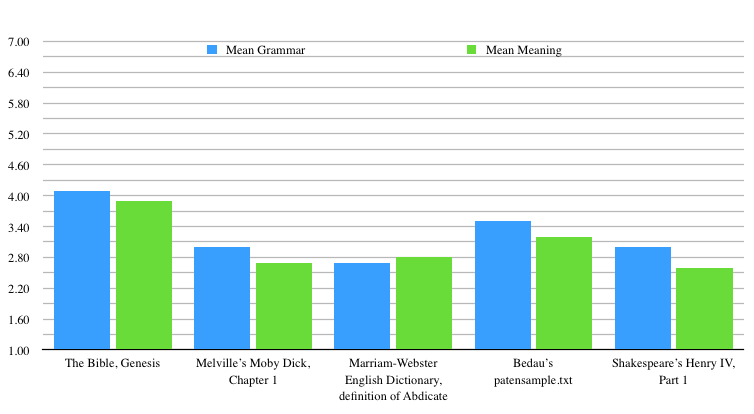
\includegraphics[width=15cm,keepaspectratio]{images/trans-diffs-grammar-meaning-chart.png}
\captionsetup{labelformat=empty} \caption{Figure 9. Chart of the differences between transcripts of the mean scores for grammar and meaning for experiments 1 and 2.}
\end{figure}

\begin{figure}[h]
\centering
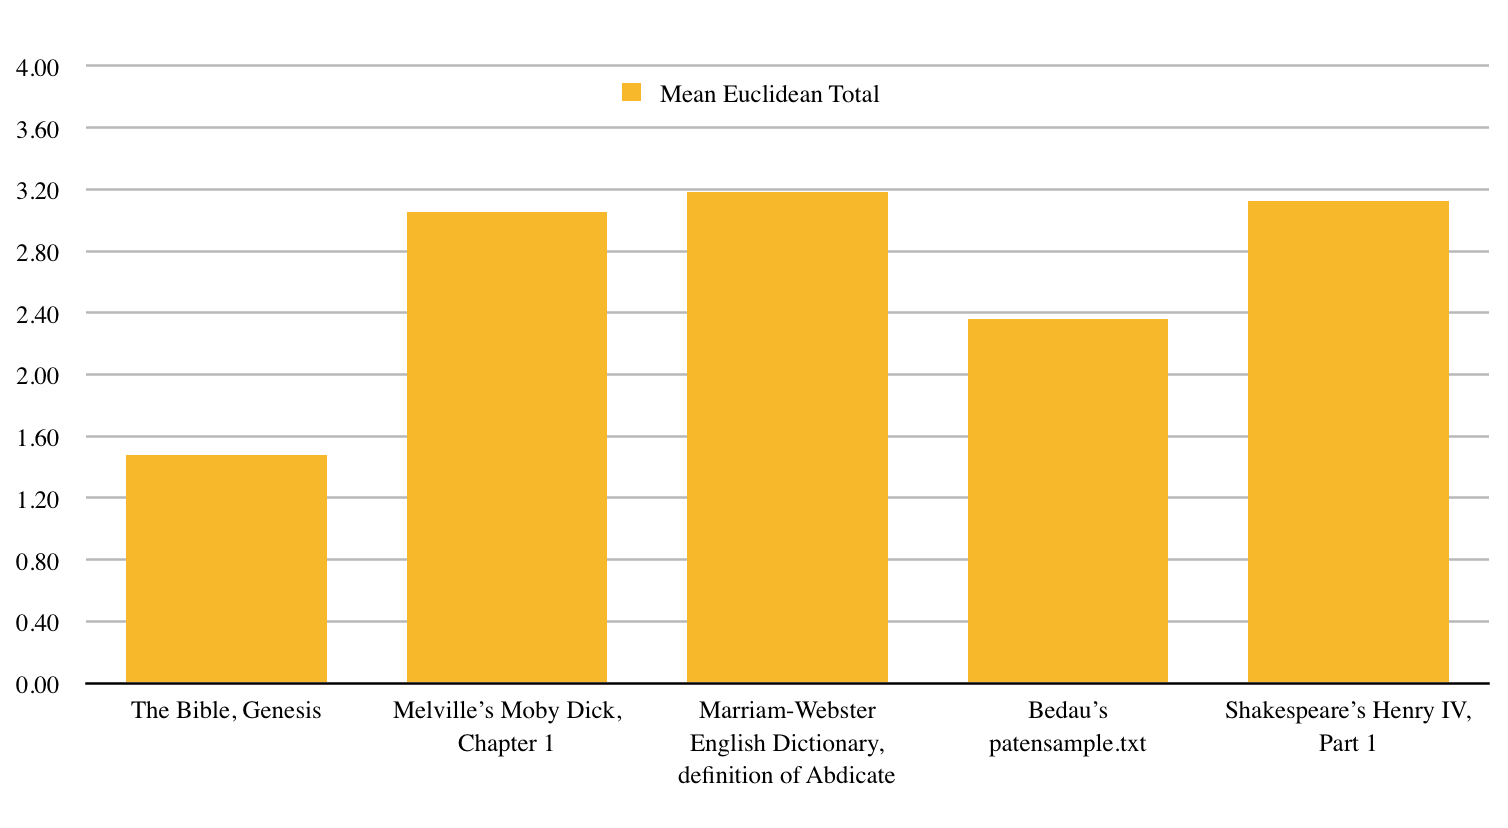
\includegraphics[width=15cm,keepaspectratio]{images/trans-diffs-euclid-chart.png}
\captionsetup{labelformat=empty} \caption{Figure 10. Chart of the differences between transcripts of the mean Euclidean total scores for experiments 1 and 2. Note that the difference of mean Euclidean total scores are negative because a smaller Euclidean total is a better score.}
\end{figure}



The Bible certainly was translated the best by far. I'd suggest that it is because the section was the shortest and has short sentences, so I may have been systematically biased in my subjective scoring because there is less space for GT to make a serious error. However the Bible translations were comparatively excellent in experiment 2 in the context GT's performance of the other texts in experiment 2, the this result does seem legitimate to some degree.





patentsample.txt scored middling, but Moby Dick, the Dictionary, and Shakespeare all scored the worst within a close range. Moby Dick and Shakespeare support my original hypothesis that these older-styled texts would be more difficult to translate, but with the Bible being a strange outlier. The Dictionary was relatively unexpected by my hypotheses, and while reading the processed texts I noticed that many of the words in the definition of abdicate, such as ``relinquish,'' were commonly switched out for something irrelevant. Additionally, the semi-colon-connected lengthy sentence of the definition is certainly uncommon in the context of most of the kinds of text I would guess that GT is trained on.


\section{Conclusions}


The results well support my original hypothesis that GT would perform better on languages with many native speakers as opposed to less. Along with the assumption that the number of native speakers correlates roughly with the amount of information for GT to train on, this confirmation suggests that the GT training process does indeed improve its performance with more data - a piece of evidence that GT works as advertised and that neural networks (part of GT's training algorithm) work well for translation.





GT had no problems translating an English translation of the Bible, which was a surprise. Perhaps the style of religious, biblical language has echoes in the texts used for other languages and lead to GT having relatively more experience translating this style. Or, perhaps more likely, the Bible has been translated into many other languages including all of those used in experiment 2 and so GT has already seen text almost exactly similar to the Bible.





GT had special problems with the definition of abdicate, Shakespeare and Moby Dick. The old-English style of writing in Shakespeare and Moby Dick apparently had great effect on GT's ability to translate grammatical structure and make sense of words that have several possible meaning, leading GT to form incorrect structures with irrelevant words. as for the definition of abdicate, this was also the case as well as the uncommon grammatical structure of a dictionary definition turning into sentence fragments or sometimes just nonsense in some trials of experiment 2.





Altogether, these observations point the conclusions that GT works better the more recent textual data it has to train on, and that artsy writing styles can severely handicap machine translation. Since this sort of data is become more and more available --- more available than ever before --- GT will likely continue to improve in commonly-used languages such as English and the languages in experiment 1. However, since data for lesser-used languages such as those in experiment 2 are not produced at the same rate, the performance gap between experiment 1 languages and experiment 2 languages is likely to increase. This does not take into account tangential breakthroughs in machine translation though, which also seem very likely; this is merely one factor in a complex formula for the future of GT. I suspect that progress in machine translation algorithms themselves will have a much larger impact on GT's future success, for much of the textual data available may not currently be of optimal training use, as demonstrated by GT's relative failure with the patentsample.txt transcript.



\forcenewpage
\section{Appendix}\subsection{Transcript: The Bible, Genesis}

Original transcript:

\begin{displayquote}
Genesis 1:1  In the beginning God created the heaven and the earth.
Genesis 1:2 And the earth was without form, and void; and darkness was upon the face of the deep. And the Spirit of God moved upon the face of the waters.
Genesis 1:3 And God said, Let there be light: and there was light.
Genesis 1:4 And God saw the light, that it was good: and God divided the light from the darkness.
Genesis 1:5 And God called the light Day, and the darkness he called Night. And the evening and the morning were the first day.
\end{displayquote}\subsubsection{Experiment 1}

Processed transcripts for each trial:

\begin{enumerate}
\item 
Genesis 1: 1 In the beginning God created the heavens and the earth.
Genesis 1: 2 There is no way on the earth, no, the darkness is deep. God's spirit moves in water.
Genesis 1: 3 God said that there is light and light.
Genesis 1: 4 God saw the light, and it is good. God separated from the darkness.
Genesis 1: 5 God calls light to tomorrow, and the darkness is called darkness. The first day is afternoon and tomorrow.


\item 
Genesis 1: 1 In the beginning God created the heavens and the earth.
Genesis 1: 2, the earth has no form, they are empty, dark and dark. The Spirit of God in the water.
Genesis 1: 3 God says to be bright and light.
Genesis 1: 4 God saw that the light was good. God divides light into darkness.
Genesis 1: 5 God calms the light of blasphemy, and darkness is night. At night and early in the morning it is the first day.


\item 
Genesis 1: 1 In the beginning God created the heavens and the earth.
Genesis 1: 2 has no form on the ground, void, darkness is darkness. The Spirit of God is in the water.
Genesis 1: 3 3 God said there is light and light.
Genesis 1: 4 God saw that light is good, and God divides light into darkness.
Genesis 1: 5 God called the light day, and the darkness of the night to tell him, and told him the night. Afternoon and dawn are the first day.


\item 
Genesis 1: 1 In the beginning God created the heavens and the earth.
Genesis 1: 2 There is no way on the earth, no, the darkness is deep. God's spirit moves in water.
Genesis 1: 3 God said that there is light and light.
Genesis 1: 4 God saw the light, and it is good. God separated from the darkness.
Genesis 1: 5 God calls light to tomorrow, and the darkness is called darkness. The first day is afternoon and tomorrow.


\item 
Genesis 1: 1 In the beginning, God created the heavens and the earth.
Genesis 1: 2 2 This earth has no shape or a hole. Dark is dark. God's spirit moves in water.
Genesis 1: 3 3 God said that there is light and light.
Genesis 1: 4 God saw the light, it is good. God separates the light from the darkness.
Genesis 1: 5 God called the light day, call the dark night. The first day is afternoon and tomorrow.

\end{enumerate}\subsubsection{Experiment 2}

Processed transcripts for each trial:

\begin{enumerate}
\item 
Genesis 1: 1, God created the earth first.
Genesis 1: 2 2 Without the earth, it was nothing. And deep and dark faces. The Spirit of God was water.
Genesis 1: 3, God said, Let it be light. There was light.
Genesis 1: 4 4 God saw the light look good. God separates light from darkness.
Genesis 1: 5 and 5 days and darkness, met yesterday evening. It was in the morning on the first day in the evening and in the morning.


\item 
Genesis 1: 1 First, God created the heavens and the earth.
Genesis 1: 2, and the world is not a place. Darkness is in the face. The Spirit of God was given to the water.
Genesis 1: 3, 3 Let us take care of God's care.
Genesis 1: 4 God saw that Revelation was beautiful and God separated the light from the darkness.
Genesis 1: 5 God called the day that He revealed and gave darkness at night. It was evening and morning on the first day.


\item 
Genesis 1: 1 The first heaven and earth were made.
Genesis 1: 2 is a world that does not like and misses. And deep in the dark. God's Spirit came out of the water.
In Genesis 1: 3 God says to light that there is light.
Genesis 1: 4 4 God is good, because he saw the light, and God divorced the light from the darkness.
Genesis 1: 5 5 God called the days of light and dark night. Early in the morning on the first day.


\item 
Genesis 1: 1 God created heaven and earth.
Genesis 1: 2 Earth is free of charge; Is deeper Spirit of God expands in water.
Genesis 1: 3 3 God said, Be light.
Genesis 1: 4 God is good light; God separated the darkness of darkness.
Genesis 1: 5 5 God has seen the light of the night and the day of darkness. Breakfast and breakfast were the first time.


\item 
Genesis 1: 1 God created heaven and earth.
Genesis 1: 2 Earth is free of charge; Is deeper Spirit of God expands in water.
Genesis 1: 3 3 God said, Be light.
Genesis 1: 4 God is good light; God separated the darkness of darkness.
Genesis 1: 5 5 God has seen the light of the night and the day of darkness. Breakfast and breakfast were the first time.

\end{enumerate}\subsection{Transcript: Melville’s Moby Dick, Chapter 1}

Original transcript:

\begin{displayquote}
There now is your insular city of the Manhattoes, belted round by
wharves as Indian isles by coral reefs- commerce surrounds it with her
surf. Right and left, the streets take you waterward. Its extreme
downtown is the battery, where that noble mole is washed by waves, and
cooled by breezes, which a few hours previous were out of sight of
land. Look at the crowds of water-gazers there.
\end{displayquote}\subsubsection{Experiment 1}

Processed transcripts for each trial:

\begin{enumerate}
\item 
This is now your city on the island of Manhattan, surrounded by
Coral reefs of Indian islands - around business
Surfing around you, the road takes you to the water. Your butt
The center is a battery, where the waves wash great bubbles.
Air cooled, invisible a few hours ago.
The earth sees the crowd there.


\item 
Now there is space in the city of Manhattan.
In the shape of an archipelago of Indian coral, Ghat-Commerce wraps itself.
Surf to the right and left, the path takes you out of the water. Above
The center is the battery that scorpion is washed with fine waves.
The air is fresh, a few hours away.
The earth See the channels in the crowd.


\item 
There is now an island city and its area in Manhattan.
India in the form of coral reef islands, surrounded by its GATT trade.
Surf around and the road will take you out of the water. Climax
The center is a battery that washes long wavelengths of 痣
The atmosphere is cool, a few hours away.
The land sees many bathrooms.



\item 
This is now your city on the island of Manhattan, surrounded by
Coral reefs of Indian islands - around business
Surfing around you, the road takes you to the water. Your butt
The center is a battery, where the waves wash great bubbles.
Air cooled, invisible a few hours ago.
The earth sees the crowd there.



\item 
Now Manhattan is their isolated city
Indian islands as a coral reef - trade around
Explore. Around, the road takes you to the surface. Its extreme
Downtown is battery, this is good mole dust, and
Air-cooled, few hours from the scene
Earth View the crowd there

\end{enumerate}\subsubsection{Experiment 2}

Processed transcripts for each trial:

\begin{enumerate}
\item 
Now that you have around your house for manatetotoko
As business coral reefs around the islands
Side. Get right and left, take waterways. Many more
The battery was the city of the shipwreck
Very low breathing, a few hours ago, blind
See the big eyes of the earth.


\item 
Now there is a belt from Manito, Einstein
Whales as large islands
Surf. To the right and to the left. margin
In the center of the city, where is the Nobel molecular molecules of batteries
The Brussels Philosopher's Breaking Down channel a few hours ago
Land. Look at the magnitude of water.


\item 
Now the city is myanattaxa, this is the zone
Coral repairs in Ailialsa vvveva as brought with you
Surf. Right and left to increase the route. nice
Battery in the city center, where the most beautiful molecules
Brejsale thikepachi, a few hours ago, picked up the vision
On the ground. Look at the masses, there is water.


\item 
Now the city of Manhattan Island
Coral Islands, they sell
Surf. Right and water on the left. Margin
Mediterranean is a well established garden
He never seen before
The ground See the crowd.


\item 
Now the city of Manhattan Island
Coral Islands, they sell
Surf. Right and water on the left. Margin
Mediterranean is a well established garden
He never seen before
The ground See the crowd.

\end{enumerate}\subsection{Transcript: Marriam-Webster English Dictionary, definition of Abdicate}

Original transcript:

\begin{displayquote}
To surrender or relinquish, as sovereign power; to withdraw
definitely from filling or exercising, as a high office, station,
dignity; as, to abdicate the throne, the crown, the papacy.
\end{displayquote}\subsubsection{Experiment 1}

Processed transcripts for each trial:

\begin{enumerate}
\item 
Discard power or sovereignty;
Complete or practice as a large office, station,
Dignity, throne raised, crown, pope


\item 
Surrender or sacrifice in the form of sovereign authority;
Obviously, when filling or practicing high level positions,
Karama, like the throne, the crown, renounced the pope.


\item 
Surrender or sacrifice in the form of a sovereign authority;
Of course, fill or exercise high, stand up,
Dignity as to the throne, crown, leaving the pope.



\item 
Discard power or sovereignty;
Complete or practice as a large office, station,
Dignity, throne raised, crown, pope



\item 
Surrender or sacrifice as surrender authority;
Of course, to fill or exercise, such as a large office, station,
Dignity, like, to give a throne, crown, pope

\end{enumerate}\subsubsection{Experiment 2}

Processed transcripts for each trial:

\begin{enumerate}
\item 
Dedication or excessive energy removal. retreat
Overall, or as a certain lengthy process,
Price, throne, crown, pope.


\item 
As a suicide or great central power. Fall
The maximum space for the office, or the suitability center
Poor sacrifice, throne, crown, pope.


\item 
Rilayaksa suicide or global power? extract
Obviously, integration or exercise, the  t
As soon as you repent the poor victims, throne, crown.


\item 
A major force to commit commitment or suicide. Remove
The highest position of office, charging, or placement clearly
Shadow Crowns, Crowns, Crowns Out.


\item 
A major force to commit commitment or suicide. Remove
The highest position of office, charging, or placement clearly
Shadow Crowns, Crowns, Crowns Out.

\end{enumerate}\subsection{Transcript: Bedau’s patensample.txt}

Original transcript:

\begin{displayquote}
To provide a polypeptide having ceramidase activity, and a gene encoding thereof useful as an reagent for lipid engineering and as indices for diagnosis of atopic dermatitis, an easy method for detecting the polypeptide and method for detecting the gene as well as a method for detecting atopic dermatitis. A polypeptide having an amino acid sequence as shown in SEQ ID NO: 1 in Sequence Listing, or a polypeptide having an amino acid sequence which has substitution, deletion, addition or insertion of one or more amino acids in the amino acid sequence of SEQ ID NO: 1 and having ceramidase activity; a gene encoding the polypeptide; a gene capable of hybridizing with the above genes under stringent conditions, and encoding a polypeptide having ceramidase activity; an oligonucleotide probe or primer, which is capable of hybridizing under stringent conditions with the above genes or with a gene having a nucleotide sequence complementary thereto; a method for detecting a gene encoding a polypeptide having ceramidase activity, by using the oligonucleotide probe and/or primer; an antibody or a fragment thereof, which is capable of specifically binding to the polypeptide; a method for detecting a polypeptide having ceramidase activity, by using the above antibody or fragment thereof; a method for detecting atopic dermatitis, by the methods. 
\end{displayquote}\subsubsection{Experiment 1}

Processed transcripts for each trial:

\begin{enumerate}
\item 
The current invention provides a peptide-containing serumidase and denatur gene activity, which can be used as a diagnostic index for the swelling of an engineered lipid reactor and atopic dermatitis, a simple method for detecting polypeptides, One way to detect genes and asymptomatic testing. Method of dermatitis In the sequence list, the SEQ ID is a amino acid sequence in the amino acid sequence described in NO: 1, or polypeptide in which the SEQ ID number 1: 1 contains optional or additions or extinction or additions to the amino acid sequence. 1 is the activity of serumides; Polypeptide encoding a gene; A gene that is capable of hybridizing the above genes in strict conditions and ceramidase activity to crack polypeptide; A small nucleotide probe or primer is able to undergo strict hybridization conditions described above or a gene with a nucleotide sequence. One method to detect genes is a pyramidal activity that is using a micro-nucleotide probe. And / or primer, an antibody or part, a method which is particularly capable of binding to polypeptide, a method to detect the activity of polypeptide using the above-known antibody or its part using semimedes There is a method, and there is a method to find out. Etopic dermatitis on the way.


\item 
Activity Sseremidejh is provided by the polypeptide and the encoding genes, a diagnosis of inflammation, as an indicator of fatty fatty acids and atopic dermatitis is a useful and simple method for detecting the gene for the detection methods of atherosclerosis found by peptides. Multiple peptide dermatitis, which contains the amino acid sequence shown in SEQ ID 1, or the amino acid sequence, contains alternatives to the removal, addition or inclusion of one or more amino acids in the polypeptide sequence. A gene encoding the polypeptide, which may be the above gene, and the activity of the Ancomaidej gene encoding the polypeptide that vibrates under stringent conditions; probe or oligonucleotide primer, which is capable of the gene or nucleotides described above. A few nucleotides and / or detection coding primers, a sequence complementary hybridization of gene therapy under stringent conditions or antibodies in which a portion, in particular, is capable of binding the polypeptide or using antibodies listed above. Part of this, a polyimin, is a way to detect cirin activity, a way to detect atopic dermatitis in some way.



\item 
The Sirimaraz activities provides polypeptides as well as genetically engineered fatty acid that code for Laid's diagnostic indicator of inflammation should be a beneficial agent, which is a simple method of detecting polypeptides and genes. Methods of detection as well as methods for detecting atopics. Inflammation of the skin is the amino acid sequence of the peptide, as shown in SEQ ID No. 1, which contains a peptide or is substituted, deleted, added, or the sequence addition of an amino acid in the amino acid sequence in the SEQ. ID. NO: 1 and ceremony activity; Polypeptide-encoding gene; capable of hybridizing under stringent conditions with the aforementioned gene, and the activity of the encoded polypeptide; Oolegnukluotad test or primer, capable of hybridizing to the aforementioned gene or gene therapy with a gene encoding a polypeptide of complementary nucleotide sequences Manner Sirimadez detection activity using the small screen oligonucleotide and / or a gene for introduction of the antibody device or a portion thereof, which may be attached, in particular, peptide material, using the antibody or fragment thereof, is a method for detecting Serimidase starch polymytoid; methods for the detection of atopic dermatitis.


\item 
The current invention provides a peptide-containing serumidase and denatur gene activity, which can be used as a diagnostic index for the swelling of an engineered lipid reactor and atopic dermatitis, a simple method for detecting polypeptides, One way to detect genes and asymptomatic testing. Method of dermatitis In the sequence list, the SEQ ID is a amino acid sequence in the amino acid sequence described in NO: 1, or polypeptide in which the SEQ ID number 1: 1 contains optional or additions or extinction or additions to the amino acid sequence. 1 is the activity of serumides; Polypeptide encoding a gene; A gene that is capable of hybridizing the above genes in strict conditions and ceramidase activity to crack polypeptide; A small nucleotide probe or primer is able to undergo strict hybridization conditions described above or a gene with a nucleotide sequence. One method to detect genes is a pyramidal activity that is using a micro-nucleotide probe. And / or primer, an antibody or part, a method which is particularly capable of binding to polypeptide, a method to detect the activity of polypeptide using the above-known antibody or its part using semimedes There is a method, and there is a method to find out. Etopic dermatitis on the way.



\item 
Ceramide to containing active polypeptide, and encrypt a method to determine the diagnostic and genetic Reactive Atrophic Atrophic Index fat inflammation, polypeptide a simple method and atopic dermatitis method to locate genes and detection. ID includes Sikyu ID shown in the polypeptide amino acid sequence of Table 1 or a sequence of peptides consisting of polyethylene replacement, deletions or additions Sikyu ID number: one or two amino acid sequence of amino acids over a plurality of amino acids Sequence: After an activity and ceramide; Gene peptide symbol. The brief stages of the gene that compress the peptide and poly hybrid under the above active parametrics; Short oligonucleotide probe or primer, which is able to complement the aforesaid gene under conditions of stringent hybridization above gene or nucleotide sequence; Gene Symbol Detection mode Poly active peptide, which is Srmadejh, a small oligonucleotide probes and / or antibodies primer or her part, and, in particular, be able to connect to the step by step; The method of detection of a polypeptide material by using the Sermode Polycarbonate activated, antibody or its part; Detection of the atopic dermatitis by the method.

\end{enumerate}\subsubsection{Experiment 2}

Processed transcripts for each trial:

\begin{enumerate}
\item 
Ceramidase marker, an easy way to find the polypeptide, and how to judge the weight of the lipidmotor treatment disease and to help atopy and atopic dermatitis is based on the polypeptide gene symbol including how dermatitis. One or more amino acid residues of a polypeptide or a secretary polypeptide sequence number of legs ID 1 list of a series of amino acids removed or replaced, including yellow installed, the list containing the amino acids. Secretary General Identification Number: 1 With sirecepta function. A collection of polypeptide components. He was able to encode a simemaraija polypeptide with difficult conditions and genetic analysis in; A high genetic sthitiharu or gas under the oligonucleotide probe or primer sequence nyukliyotedisa the bottom of the sink; software oligonucleotide and / or primer, how to use the components to produce siremaidesa synthetic polypeptide; An integer or piece of it combines its immediate popppaidama. The process to be used to find popipippaida work siremaidasa high anti-piece or pieces of them; How to Treat Atopic Skin Diseases.


\item 
Ceramics polypeptide function using one polypeptide and function on the system and used as a diagnostic lipid and atopic dermatitis is an epimeric legal method to see genetic skin diseases. The list of peptide foot sequences Popeipidide identity Secretary over ID on the sequence of the sequence: No: 1 and one or more ammunition ceramic function: Number of ID General Sport amino acid, including 1 ID SEO, or peptide. Genetic coding polypeptide. Hybridizing genetic material can be a powerful sign that leads Ceramic polypeptide genetic material and high quality standards. Completing a single series of oligonucleotide tests or hybridizing disruption, means genetic or weight under difficult conditions. 1. oligonucleotide and / or primer using a method of ceramidase polypeptide function. Buddhism, especially the body or can be tied to polypeptide. each method is exposed to polypeptide containing antibodies against the ceramide or part. Another way for atopic skin diseases.


\item 
The polypeptide is used as a recovery agent that detects lipid epidermis and mechanical activities, and makes Siremaraya, a polypeptide, and an atopy to easily find a way to cope with the genetic predisposition of skin symptoms. No: 1 List of Legs or Foot Popipipidae Foot Ennio Acid Sole, One or More Amino Acids including Numbers Illustrated Mobile Polypeptide. An improved condition for the enhancement of the genetic genetic material, the polypeptide code, and the hybridization function of siremades. Investigation of oligonucleotides or primers with a hybrid genetic component to complete the genetic function and the status of complex nucleotide sequences. oligonucleotide probes and / or the detection of cerebral ceramide primers, in particular binding of the polypeptide function of the body or fragment. The immune system or polypeptide used to determine the activity of the susceptible system. Atopic pathology.


\item 
keramiasis work and find atopic polypeptide in lipid engineering and genes that find easy way to detect and detect dermatitis disease diagnosis, polypyipideide and atopic gene. Armæṭēsis. Secretary 1. Popipyipideide acidic acid acid sequence is without foot: 1, any one or more anemic acid removed from any id or secretary removed or connected to peptipide. 1 and operation of ceramide. A symbol which represents polypeptide. Genetic material is capable of hybridizing under genetic state and cinemorridge representing peptipidide. In difficult situations, finding out how to represent a component or primer primer using this whole nucleotide sequence or genetic and genetic examination oligonulated and / or primer ceramade function hybridized popped research. If you have the capability, the immune system makes the right to poppeptide or Buddhist religion. Body or polypeptide with a piece of keramiasis to find a way. The process to identify unemployed dematatitis.


\item 
keramiasis work and find atopic polypeptide in lipid engineering and genes that find easy way to detect and detect dermatitis disease diagnosis, polypyipideide and atopic gene. Armæṭēsis. Secretary 1. Popipyipideide acidic acid acid sequence is without foot: 1, any one or more anemic acid removed from any id or secretary removed or connected to peptipide. 1 and operation of ceramide. A symbol which represents polypeptide. Genetic material is capable of hybridizing under genetic state and cinemorridge representing peptipidide. In difficult situations, finding out how to represent a component or primer primer using this whole nucleotide sequence or genetic and genetic examination oligonulated and / or primer ceramade function hybridized popped research. If you have the capability, the immune system makes the right to poppeptide or Buddhist religion. Body or polypeptide with a piece of keramiasis to find a way. The process to identify unemployed dematatitis.

\end{enumerate}\subsection{Transcript: Shakespeare’s Henry IV, Part 1}

Original transcript:

\begin{displayquote}
My liege, this haste was hot in question,
And many limits of the charge set down
But yesternight: when all athwart there came
A post from Wales loaden with heavy news;
Whose worst was, that the noble Mortimer,
Leading the men of Herefordshire to fight
Against the irregular and wild Glendower,
Was by the rude hands of that Welshman taken,
A thousand of his people butchered;
Upon whose dead corpse there was such misuse,
Such beastly shameless transformation,
By those Welshwomen done as may not be
Without much shame retold or spoken of.
\end{displayquote}\subsubsection{Experiment 1}

Processed transcripts for each trial:

\begin{enumerate}
\item 
God, this haste problem is very hot,
And many more restrictions.
But tonight: when everyone is here.
There are several new features in an article in Wales.
Worst, who is the great mortimer,
Bring people here to fight
Against irregular and wild glow,
She was taken with the shameless arm of Welsh.
One thousand of them were massacred.
The bodies are such violations.
It's a shameful change
Perhaps for these Welsh women.
There is not much shame in repeating or saying.


\item 
As a liar, this question is very hot,
We have established many billing limits
But calm: when all athletes come.
Wales publications are full of breaking news;
The worst is the great dead.
The leaders go to Hereford to fight.
Irregular irregular glow,
This is Wilchman's strong hand.
There are a thousand butchers.
Who damages your body?
This shameful change
It can be done by a Welsh woman who can not afford it.
There is not much shame, retirement or conversation.



\item 
My lie, this craze is very hot on this issue,
Pregnancy is subject to many restrictions.
But serenity: when all the athletes are coming.
The Welsh post is full of breaking news.
The worst is Mortimer's greatness.
These people were taken to Hereford to fight
Fighting irregularities and wild glow
Take a hard Welsh hand,
A butcher of a thousand people.
Who has been misused by your body?
These obvious changes,
This can be done by a Welshman who can not
Not too shy, retiring or talking.


\item 
God, this haste problem is very hot,
And many more restrictions.
But tonight: when everyone is here.
There are several new features in an article in Wales.
Worst, who is the great mortimer,
Bring people here to fight
Against irregular and wild glow,
She was taken with the shameless arm of Welsh.
One thousand of them were massacred.
The bodies are such violations.
It's a shameful change
Perhaps for these Welsh women.
There is not much shame in repeating or saying.



\item 
As a lie, the craze over the issue is very hot.
And it offers many restrictions
But last night: all the ramps are coming on.
News published in Wales is full of important news;
Worst, Mortimer is great,
Ordering fighters of Herefordshire
Against irregular and wild glue,
I have a Welsh monk
One thousand of them were killed.
There the body was abused,
It's a shameful and cruel change
What can be done by those vilgium is not
There is no shame listed or spoken.

\end{enumerate}\subsubsection{Experiment 2}

Processed transcripts for each trial:

\begin{enumerate}
\item 
My sleep was a sudden heat
And many other criminal cases have been identified
At night, everything from and close
Welle positions are tricky questions.
Horse, good mortar,
The struggle for the people of yahaundaphordasayarama
Unusual glendavara and dry,
They hit by vellyandako
Thousands of people were killed.
When their body is persecuted,
This is an important translation
The same is true of women in Wales
Shame or needless to mention.


\item 
A liar, chest in the chest,
There are many numbers set
But do not enter: where all artists come
Full of English with full space;
and
More Arferdshire men fought
Whether it's inappropriate or wild,
Watch Valentine's wonders,
Thousands have been raped.
What kinds of abuse on these devices,
Such a change,
Wales
Talking too much.


\item 
My lie and my chest were hot with this problem
And the money was banned many times
But yirnerne: where the artists come from
Loading weight avatar avatar
then
Men fight for airbags
Unusual and clever wildlife,
He wanted a great talent
Thousands of people fell.
What is their carcass?
Such changes are abusive bessandeha
As Welsh Women Can Do
Talk more without talking.


\item 
This was my question of disappointment
There are many limitations for the award
But at night, when all the tourists arrive
The Polish message was completely opened in Welsh.
Gentlemen,
Hufffordshire people were fighters
Wenjing and Wenzhou against Glenn
To bring a Welsh Welsh hand,
Thousands of people are killed.
Such a type of body was abusive.
Without migration, such horrible,
Welsh, Yo
It's not embarrassing to back or chat.


\item 
This was my question of disappointment
There are many limitations for the award
But at night, when all the tourists arrive
The Polish message was completely opened in Welsh.
Gentlemen,
Hufffordshire people were fighters
Wenjing and Wenzhou against Glenn
To bring a Welsh Welsh hand,
Thousands of people are killed.
Such a type of body was abusive.
Without migration, such horrible,
Welsh, Yo
It's not embarrassing to back or chat.

\end{enumerate}



\end{document}